%%%%%%%%%%%%%%%%%%
%%%   Template para utilização do plano de estágio %%%
%%%%%%%%%%%%%%%%%%

%% Preencher apenas os dados entre {}

\documentclass[12pt,openright,oneside,a4paper,english,french,spanish,brazil]{unifil}
\usepackage{float}
\usepackage{needspace}

% O abntex2 separa o rótulo da legenda com travessão (\ABNTEXcaptiondelim vale
% ~\textendash~). Trocado por dois-pontos.
\renewcommand{\ABNTEXcaptiondelim}{:~}

\titulo{RESERVA DE SALAS} 
\autor{JOSÉ RONALDO DOS SANTOS JÚNIOR} % Nome do aluno
\instituicao{Centro Universitário Filadélfia}
\local{Londrina}
\data{2026} % Ano de publicação
\preambulo{Curso de bacharelado em Ciência da Computação} % Nome do curso
\orientador{GUSTAVO QUEIROZ SILVEIRA} % Nome do orientador
\input{../../../out/drive-links.tex}

% A NBR 6023:2018 tirou os sinais < > em volta do endereço, que a edição de 2002 exigia. O
% abntex2cite ainda aplica a forma antiga em todo \url do documento. Isto desfaz, e vale
% também para as referências, que precisam seguir a mesma edição da norma que as figuras.
\def\UrlLeft{}\def\UrlRight{}

% Fonte de figura cuja versão vetorial está no Drive, no formato da ABNT NBR 6023: endereço
% depois de "Disponível em:" e data depois de "Acesso em:". O argumento é uma macro de
% out/drive-links.tex, nunca a URL escrita à mão. O \expandafter faz a macro virar texto
% antes de o \url recebê-la, que é o que permite quebrar o endereço no fim da linha.
\newcommand{\fonteDrive}[1]{%
  {\footnotesize \textbf{Fonte:} O autor.
   Disponível em: \expandafter\url\expandafter{#1}. Acesso em: 1 nov. 2026.}}

\begin{document}

\frenchspacing

%%%%%%%%%%%%%%%%%%%%%%%%%%%%
%% Elementos pré-textuais %%
%%%%%%%%%%%%%%%%%%%%%%%%%%%%

\pretextual


%Campo de inclusão dos capítulos que complementam o Plano de Estágio
\imprimircapa

%%Não mexer

\tableofcontents*

  \setlength\absleftindent{0cm}
  \setlength\absrightindent{0cm}
  
  %fonte do ambiente%
  \abstracttextfont{\normalfont\normalsize}

  %indentação e espaçamento entre parágrafos%
  \setlength{\absparindent}{0pt}
  \setlength{\absparsep}{18pt}


\textual

\renewcommand{\ABNTEXchapterfont}{\fontfamily{cmr}\fontseries{b}\selectfont}
\renewcommand{\ABNTEXchapterfontsize}{\Large}

\renewcommand{\ABNTEXsectionfont}{\uppercase{\fontfamily{cmr}\fontseries{b}\selectfont}}
\renewcommand{\ABNTEXsectionfontsize}{\large}

%Inclusão dos capítulos que fazem parte do plano de estágio

% Organização sugerida para uma introdução de relatório de estágio

\chapter{Introdução}\label{sec:1}

% \textbf{(MÍNIMO UMA PÁGINA)}

% A introdução do trabalho deverá contextualizar a proposta de desenvolvimento do estágio. 

% Contextualizar deve ser entendido aqui como uma explicação de como o acadêmico chegou à esta proposta de estágio supervisionado.

% Lembre que na introdução de seu trabalho a seguinte pergunta deverá ser  respondida ao leitor : “se eu continuar a ler o trabalho daqui para frente o que vou encontrar no seu texto?”

% Exemplo:

% (resumido e fictício apenas para fins de exemplo)

% “A Lei Complementar no 101, de 4 de maio de 2000, intitulada Lei de Responsabilidade Fiscal - LRF,
% estabelece normas de finanças públicas voltadas para a responsabilidade na gestão
% fiscal, mediante ações em que se previnam riscos e corrijam desvios capazes de afetar o
% equilíbrio das contas públicas, destacando-se o planejamento, o controle, a
% transparência e a responsabilização como premissas básicas.” Tesouro Nacional, 2008

% A partir da publicação da LRF ficou evidente que a utilização de recursos
% tecnológicos para acompanhamento da gestão se faz necessária nas diversas
% esferas do poder público.

% ...

% O presente projeto de estágio propõe a análise e o desenvolvimento de uma
% aplicação de controle orçamentário para a Prefeitura Municipal do Vale dos Sonhos.

% O projeto de estágio descreve os objetivos do trabalho, detalha a proposta do
% sistema a ser desenvolvido, faz um breve resgate da teoria que ampara o sistema
% proposto e apresenta o cronograma e ferramental de hardware e software estimado
% para o desenvolvimento do trabalho.

% \section{PROPOSTA E OBJETIVOS}

%Quais objetivos (geralmente 1 objetivo geral e no mínimo 5 específicos) o acadêmico pretende atingir com o desenvolvimento do estágio.

% Evite aqui objetivos como: “o objetivo deste trabalho é concluir o curso de
% graduação”, o objetivo a ser abordado neste tópico é o objetivo do sistema proposto.


% Exemplo (resumido e fictício apenas para fins de exemplo)

%    O presente projeto tem como objetivo principal (ou objetivo geral) propor uma
% solução de acompanhamento do orçamento do município de Vale dos Sonhos.
% Como objetivos específicos o sistema irá proporcionar a o cadastramento e a consulta do orçamento municipal aprovado pela Câmara de Vereadores de Vale dos
% Sonhos, tão bem quanto o acompanhamento on-line dos empenhos e pagamentos
% efetuados

% (os objetivos gerais e específicos poderão ser feitos na forma de tópicos se melhor convier ao aluno)

% \section{JUSTIFICATIVA}

% Qual é a proposta do seu sistema? Como (e porque) ela se justifica como uma proposta válida?

% Neste item você dever fazer uma breve descrição do seu sistema (proposta) e porque ele é importante para a empresa cedente (justificativa).

% Exemplo :

% (este exemplo está resumido e é fictício)

% O sistema proposto permitirá o controle dos gastos públicos por meio da inclusão dos pagamentos efetuados pelo setor financeiro da Prefeitura do Vale dos Sonhos disponibilizando o acesso ao orçamento municipal imediatamente aos contribuintes que efetuarem consultas na Internet. (PROPOSTA)

% “A LRF cria condições para a implantação de uma nova cultura gerencial na gestão dos recursos públicos e incentiva o exercício pleno da cidadania, especialmente no que se refere à participação do contribuinte no processo de acompanhamento da aplicação dos recursos públicos e de avaliação dos seus resultados”, desta forma o presente projeto se justifica por atender a uma demanda da Prefeitura Municipal de Vale dos Sonhos buscando a transparência na gestão dos recursos públicos do município. (JUSTIFICATIVA)


Uma instituição de ensino superior enfrenta diversos desafios administrativos para poder garantir uma boa qualidade no ensino oferecido. O avanço da tecnologia da informação vem proporcionando diversas melhorias para a otimização de processos administrativos, com redução de falhas, riscos e custos operacionais.

Em função do tempo o gerenciamento de salas de uma instituição de ensino pode acabar se tornando uma tarefa complexa, devido às necessidades como as trocas de horários, alta demanda e controles de restrições. Assim, processos realizados de forma manual como a utilização de planilhas podem acabar resultando em conflitos de agendamento, retrabalho e dificuldades no acompanhamento das reservas realizadas.

O presente relatório de estágio descreve o desenvolvimento realizado de uma aplicação de controle de agendamentos de salas para o Núcleo de Prática de Informática - NPI.

Este relatório descreve os objetivos alcançados, detalha os casos de uso implementados, os recursos e o ambiente de desenvolvimento utilizados, bem como os resultados obtidos ao longo do estágio.

\section{PROPOSTA E OBJETIVOS}

% O presente projeto tem como objetivo principal (ou objetivo geral) propor uma solucao de agendamento de salas para a unifil. o Sistema irá proporcionar controle de resolução de conflito e cadastros de salas e usuários, controle de históricos de alterações, uma agenda centralizada da locação dos recursos e geração de relatórios.

principal (ou objetivo geral) desenvolver uma solução de agendamento de salas para a UniFil. Os seus objetivos específicos foram:

\begin{itemize}

    \item \textbf{Padronizar o fluxo de reserva}, estabelecendo um caminho único de
          solicitação, análise e confirmação, com estados explícitos para cada
          solicitação.

    \item \textbf{Automatizar a verificação de disponibilidade}, apresentando ao
          solicitante apenas as salas livres no período desejado, filtradas por
          capacidade, prédio, tipo de sala e recursos.

    \item \textbf{Detectar conflitos de agendamento pelo sistema}, verificando a
          sobreposição de horários no momento do envio da solicitação.

    \item \textbf{Registrar o histórico das decisões} tornando possível reconstruir o que
          foi decidido, por quem e quando.

    \item \textbf{Disponibilizar relatórios} sobre uso, agendamentos e
          histórico do sistema, com a exportação opcional do resultado em arquivo.
\end{itemize}

\section{JUSTIFICATIVA}

O sistema em desenvolvimento permite o controle de alocação de salas por meio de uma centralização das informações e automatização do processo de agendamento. O sistema está substituindo o processo anterior realizado em planilhas, garantindo maior confiabilidade e eficiência operacional.
\chapter{Diagramas}\label{sec:2}

Este capítulo apresenta os diagramas elaborados durante o desenvolvimento do sistema de reserva de salas. São abordados, entre outros, o diagrama de caso de uso, o diagrama entidade-relacionamento (DER), o diagrama de componentes e o diagrama de classes. A modelagem foi realizada com o objetivo de representar, de forma visual e estruturada, os requisitos, a arquitetura e o comportamento da aplicação.

\section{Diagrama de caso de uso}

O diagrama de caso de uso é uma das partes fundamentais do projeto, pois é com ele que serão definidos os requisitos funcionais de forma clara do sistema. Na Figura~\ref{fig:caso-de-uso} são apresentados os principais atores e funcionalidades da aplicação.

\begin{figure}[H]
    \caption{Diagrama de caso de uso do sistema de reserva de salas}
    \label{fig:caso-de-uso}
    \centering
    \includegraphics[width=0.95\textwidth,height=0.75\textheight,keepaspectratio]{../../../out/src/plantuml/usecasediagram.png}

    {\footnotesize \textbf{Fonte:} O autor.
    \textbf{Acesso:} \href{\linkUsecasediagram}{Diagrama de Caso de Uso}.}
\end{figure}

\subsection{Atores}

\begin{description}
    \item[\textbf{sa\_professor}] Representa o usuário comum do sistema. Associa-se diretamente ao gerenciamento de solicitações, de ambientes e de agendamentos, além da geração de relatórios.

    \item[\textbf{sa\_coordenador}] Especialização de \textbf{sa\_professor}, herdando todas as suas permissões. Possui acesso adicional ao gerenciamento de usuários do sistema.
\end{description}

\subsection{Casos de uso}

\begin{description}
    \item[\textbf{suc\_gerenciar\_ambientes}] Reúne o cadastro, a edição, a remoção e a consulta dos elementos que compõem o espaço físico da instituição.

    \begin{description}
        \item[\textbf{suc\_gerenciar\_prédios}] Trata dos prédios, que delimitam onde cada sala está localizada.

        \item[\textbf{suc\_gerenciar\_salas}] Trata das salas propriamente ditas, que são as unidades efetivamente reserváveis.

        \item[\textbf{suc\_gerenciar\_tipos\_de\_salas}] Trata da classificação das salas, por exemplo laboratório, auditório ou sala de aula.

        \item[\textbf{suc\_gerenciar\_recursos}] Trata dos recursos associados às salas, como projetores e computadores.
    \end{description}

    \item[\textbf{suc\_gerenciar\_agendamentos}] Permite criar, atualizar, cancelar e visualizar agendamentos de salas.

    \item[\textbf{suc\_gerenciar\_solicitações}] Permite registrar e acompanhar as solicitações de reserva, com seus respectivos status.

    \item[\textbf{suc\_gerar\_relatórios}] Permite emitir relatórios com informações consolidadas sobre uso, agendamentos e histórico do sistema.

    \item[\textbf{suc\_exportar\_relatórios}] Estende \textbf{suc\_\allowbreak{}gerar\_\allowbreak{}relatórios} com a exportação do resultado em arquivo. É um comportamento opcional: o relatório pode ser apenas consultado, sem ser exportado.

    \item[\textbf{suc\_gerenciar\_usuarios}] Permite cadastrar, editar, remover e consultar usuários do sistema.
\end{description}

\section{Diagrama de Entidade e Relacionamento}

Na Figura~\ref{fig:der} é apresentado o diagrama de entidade-relacionamento do sistema,
evidenciando as entidades, seus atributos e os relacionamentos entre elas.

\begin{figure}[H]
    \caption{Diagrama de entidade-relacionamento do sistema de reserva de salas}
    \label{fig:der}
    \centering
    \includegraphics[width=0.95\textwidth,height=0.75\textheight,keepaspectratio]{../../../out/src/plantuml/entidade-relacionamento/der.png}

    {\footnotesize \textbf{Fonte:} O autor.}
\end{figure}

\section{Diagrama de Componentes}

Na Figura~\ref{fig:componentes} é apresentada a visão geral dos módulos do sistema e das
dependências entre eles.

\begin{figure}[H]
    \caption{Visão geral dos módulos do sistema de reserva de salas}
    \label{fig:componentes}
    \centering
    % O PNG tem 257x230 px. Acima de 0,5\textwidth ele passa a ser ampliado e serrilha.
    \includegraphics[width=0.5\textwidth,keepaspectratio]{../../../out/src/plantuml/componentes.png}

    {\footnotesize \textbf{Fonte:} O autor.}
\end{figure}

\section{Diagramas de Classe}

O sistema segue uma arquitetura de módulos, cada módulo possui seu próprio domínio, casos de uso e camada de infraestrutura. Cada diagrama exibe as três camadas da arquitetura do módulo: \textbf{Domain} (entidades, objetos de valor e enumerações), \textbf{Application} (casos de uso e portas) e \textbf{Infrastructure} (controladores, repositórios e adaptadores).

\subsection{Usuário}

Na Figura~\ref{fig:classe-user} são apresentadas as classes do módulo de gerenciamento de usuários.

\begin{figure}[H]
    \caption{Diagrama de classe do usuário}
    \label{fig:classe-user}
    \centering
    \includegraphics[width=0.95\textwidth,height=0.75\textheight,keepaspectratio]{../../../out/src/plantuml/classe/simples/user_simples.png}

    {\footnotesize \textbf{Fonte:} O autor.}
\end{figure}

\subsection{Sala}

Na Figura~\ref{fig:classe-building}, Figura~\ref{fig:classe-room-type}, Figura~\ref{fig:classe-resource} e Figura~\ref{fig:classe-room} são apresentadas respectivamente as classes de \texttt{Building}, \texttt{RoomType}, \texttt{Resource} e \texttt{Room}, que compõem o módulo de gerenciamento de salas.

\begin{figure}[H]
    \caption{Diagrama de classe do prédio}
    \label{fig:classe-building}
    \centering
    \includegraphics[width=0.95\textwidth,height=0.75\textheight,keepaspectratio]{../../../out/src/plantuml/classe/simples/room/room_building.png}

    {\footnotesize \textbf{Fonte:} O autor.}
\end{figure}

\begin{figure}[H]
    \caption{Diagrama de classe do tipo de sala}
    \label{fig:classe-room-type}
    \centering
    \includegraphics[width=0.95\textwidth,height=0.75\textheight,keepaspectratio]{../../../out/src/plantuml/classe/simples/room/room_room_type.png}

    {\footnotesize \textbf{Fonte:} O autor.}
\end{figure}

\begin{figure}[H]
    \caption{Diagrama de classe do recurso}
    \label{fig:classe-resource}
    \centering
    \includegraphics[width=0.95\textwidth,height=0.75\textheight,keepaspectratio]{../../../out/src/plantuml/classe/simples/room/room_resource.png}

    {\footnotesize \textbf{Fonte:} O autor.}
\end{figure}

\begin{figure}[H]
    \caption{Diagrama de classe da sala}
    \label{fig:classe-room}
    \centering
    \includegraphics[width=0.95\textwidth,height=0.75\textheight,keepaspectratio]{../../../out/src/plantuml/classe/simples/room/room_room.png}

    {\footnotesize \textbf{Fonte:} O autor.}
\end{figure}

\subsection{Evento}

Na Figura~\ref{fig:classe-event} e Figura~\ref{fig:classe-period} são apresentadas respectivamente as classes do evento com sua solicitação de alteração e as classes do período, ambas do módulo de gerenciamento de eventos.

\begin{figure}[H]
    \caption{Diagrama de classe do evento e da solicitação}
    \label{fig:classe-event}
    \centering
    \includegraphics[width=0.95\textwidth,height=0.75\textheight,keepaspectratio]{../../../out/src/plantuml/classe/simples/event/event_and_request.png}

    {\footnotesize \textbf{Fonte:} O autor.}
\end{figure}

\begin{figure}[H]
    \caption{Diagrama de classe do período}
    \label{fig:classe-period}
    \centering
    \includegraphics[width=0.95\textwidth,height=0.75\textheight,keepaspectratio]{../../../out/src/plantuml/classe/simples/event/event_period.png}

    {\footnotesize \textbf{Fonte:} O autor.}
\end{figure}

\subsection{Relatório}

Na Figura~\ref{fig:classe-report} são apresentadas as classes do módulo de relatórios.

\begin{figure}[H]
    \caption{Diagrama de classe do relatório}
    \label{fig:classe-report}
    \centering
    \includegraphics[width=0.95\textwidth,height=0.75\textheight,keepaspectratio]{../../../out/src/plantuml/classe/simples/report_simples.png}

    {\footnotesize \textbf{Fonte:} O autor.}
\end{figure}

\section{Diagramas de Sequência}

Nesta seção são apresentados os diagramas de sequência das operações do sistema,
descrevendo o fluxo de mensagens entre os componentes. Cada figura reúne os endpoints de
um módulo, separados por blocos.

\begin{itemize}
    \item A Figura~\ref{fig:seq-user} representa as operações do módulo de gerenciamento de usuários.
    \item A Figura~\ref{fig:seq-room} representa as operações do módulo de gerenciamento de salas.
    \item A Figura~\ref{fig:seq-event} representa as operações de consulta do módulo de gerenciamento de eventos.
    \item A Figura~\ref{fig:seq-report} representa as operações do módulo de relatórios.
\end{itemize}

\begin{figure}[H]
    \caption{Diagrama de sequência do usuário}
    \label{fig:seq-user}
    \centering
    \includegraphics[width=0.95\textwidth,height=0.85\textheight,keepaspectratio]{../../../out/src/plantuml/sequencia/simples/user_simples.png}

    {\footnotesize \textbf{Fonte:} O autor.}
\end{figure}

\begin{figure}[H]
    \caption{Diagrama de sequência da sala}
    \label{fig:seq-room}
    \centering
    \includegraphics[width=0.95\textwidth,height=0.85\textheight,keepaspectratio]{../../../out/src/plantuml/sequencia/simples/room_simples.png}

    {\footnotesize \textbf{Fonte:} O autor.}
\end{figure}

\begin{figure}[H]
    \caption{Diagrama de sequência do evento}
    \label{fig:seq-event}
    \centering
    \includegraphics[width=0.95\textwidth,height=0.85\textheight,keepaspectratio]{../../../out/src/plantuml/sequencia/simples/event_simples.png}

    {\footnotesize \textbf{Fonte:} O autor.}
\end{figure}

\begin{figure}[H]
    \caption{Diagrama de sequência do relatório}
    \label{fig:seq-report}
    \centering
    \includegraphics[width=0.95\textwidth,height=0.85\textheight,keepaspectratio]{../../../out/src/plantuml/sequencia/simples/report_simples.png}

    {\footnotesize \textbf{Fonte:} O autor.}
\end{figure}

\section{Diagramas de Estado}\label{sec:estado}

Nas figuras a seguir são apresentados os diagramas de estado das entidades do sistema,
descrevendo os ciclos de vida e as transições de estado possíveis.

\subsection{Usuário}

Na Figura~\ref{fig:estado-user} é representado o ciclo de vida da entidade \texttt{User} do módulo de gerenciamento de usuários.

\begin{figure}[H]
    \caption{Diagrama de estado do usuário}
    \label{fig:estado-user}
    \centering
    \includegraphics[width=0.95\textwidth,height=0.75\textheight,keepaspectratio]{../../../out/src/plantuml/estado/user_status.png}

    {\footnotesize \textbf{Fonte:} O autor.}
\end{figure}

\subsection{Sala}

Na Figura~\ref{fig:estado-room}, Figura~\ref{fig:estado-room-type}, Figura~\ref{fig:estado-building} e Figura~\ref{fig:estado-resource} são representados respectivamente os ciclos de vida das entidades \texttt{Room}, \texttt{RoomType}, \texttt{Building} e \texttt{Resource} do módulo de gerenciamento de salas.

\begin{figure}[H]
    \caption{Diagrama de estado da sala}
    \label{fig:estado-room}
    \centering
    \includegraphics[width=0.95\textwidth,height=0.75\textheight,keepaspectratio]{../../../out/src/plantuml/estado/room_status.png}

    {\footnotesize \textbf{Fonte:} O autor.}
\end{figure}

\begin{figure}[H]
    \caption{Diagrama de estado do tipo de sala}
    \label{fig:estado-room-type}
    \centering
    \includegraphics[width=0.95\textwidth,height=0.75\textheight,keepaspectratio]{../../../out/src/plantuml/estado/room_type_status.png}

    {\footnotesize \textbf{Fonte:} O autor.}
\end{figure}

\begin{figure}[H]
    \caption{Diagrama de estado do prédio}
    \label{fig:estado-building}
    \centering
    \includegraphics[width=0.95\textwidth,height=0.75\textheight,keepaspectratio]{../../../out/src/plantuml/estado/building_status.png}

    {\footnotesize \textbf{Fonte:} O autor.}
\end{figure}

\begin{figure}[H]
    \caption{Diagrama de estado do recurso}
    \label{fig:estado-resource}
    \centering
    \includegraphics[width=0.95\textwidth,height=0.75\textheight,keepaspectratio]{../../../out/src/plantuml/estado/resource_status.png}

    {\footnotesize \textbf{Fonte:} O autor.}
\end{figure}

\subsection{Evento}

Na Figura~\ref{fig:estado-event}, Figura~\ref{fig:estado-event-request} e Figura~\ref{fig:estado-period} são representados respectivamente os ciclos de vida das entidades \texttt{Event}, \texttt{EventRequest} e \texttt{Period} do módulo de gerenciamento de eventos.

\begin{figure}[H]
    \caption{Diagrama de estado do evento}
    \label{fig:estado-event}
    \centering
    \includegraphics[width=0.95\textwidth,height=0.75\textheight,keepaspectratio]{../../../out/src/plantuml/estado/event_status.png}

    {\footnotesize \textbf{Fonte:} O autor.}
\end{figure}

\begin{figure}[H]
    \caption{Diagrama de estado da solicitação de alteração}
    \label{fig:estado-event-request}
    \centering
    \includegraphics[width=0.95\textwidth,height=0.75\textheight,keepaspectratio]{../../../out/src/plantuml/estado/event_request_status.png}

    {\footnotesize \textbf{Fonte:} O autor.}
\end{figure}

\begin{figure}[H]
    \caption{Diagrama de estado do período}
    \label{fig:estado-period}
    \centering
    \includegraphics[width=0.95\textwidth,height=0.75\textheight,keepaspectratio]{../../../out/src/plantuml/estado/period_status.png}

    {\footnotesize \textbf{Fonte:} O autor.}
\end{figure}

\subsection{Relatório}

Na Figura~\ref{fig:estado-report} é representado o ciclo de vida da entidade \texttt{Report} do módulo de relatórios.

\begin{figure}[H]
    \caption{Diagrama de estado do relatório}
    \label{fig:estado-report}
    \centering
    \includegraphics[width=0.95\textwidth,height=0.75\textheight,keepaspectratio]{../../../out/src/plantuml/estado/report_status.png}

    {\footnotesize \textbf{Fonte:} O autor.}
\end{figure}

\section{Diagrama de Implantação}

Na Figura~\ref{fig:implantacao} é apresentado o diagrama de implantação do sistema,
descrevendo a arquitetura física e a distribuição dos componentes nos nós de infraestrutura.

\begin{figure}[H]
    \caption{Diagrama de implantação do sistema de reserva de salas}
    \label{fig:implantacao}
    \centering
    \includegraphics[width=0.95\textwidth,height=0.75\textheight,keepaspectratio]{../../../out/src/plantuml/deployment.png}

    {\footnotesize \textbf{Fonte:} O autor.}
\end{figure}


\chapter{Telas}\label{sec:3}

As telas foram feitas com objetivo de serem simples e acessíveis para os usuários, além de proverem ferramentas necessárias para o uso avançado do sistema.

\Needspace{0.7\textheight}
\subsection{Tela de login}
Como demonstrado em Figura~\ref{fig:tela-login}, serão solicitadas ao usuário suas credenciais, no caso, o seu e-mail e senha para acesso.

\begin{figure}[H]
    \caption{Tela de login}
    \label{fig:tela-login}
    \centering
    \makebox[\textwidth][c]{%
        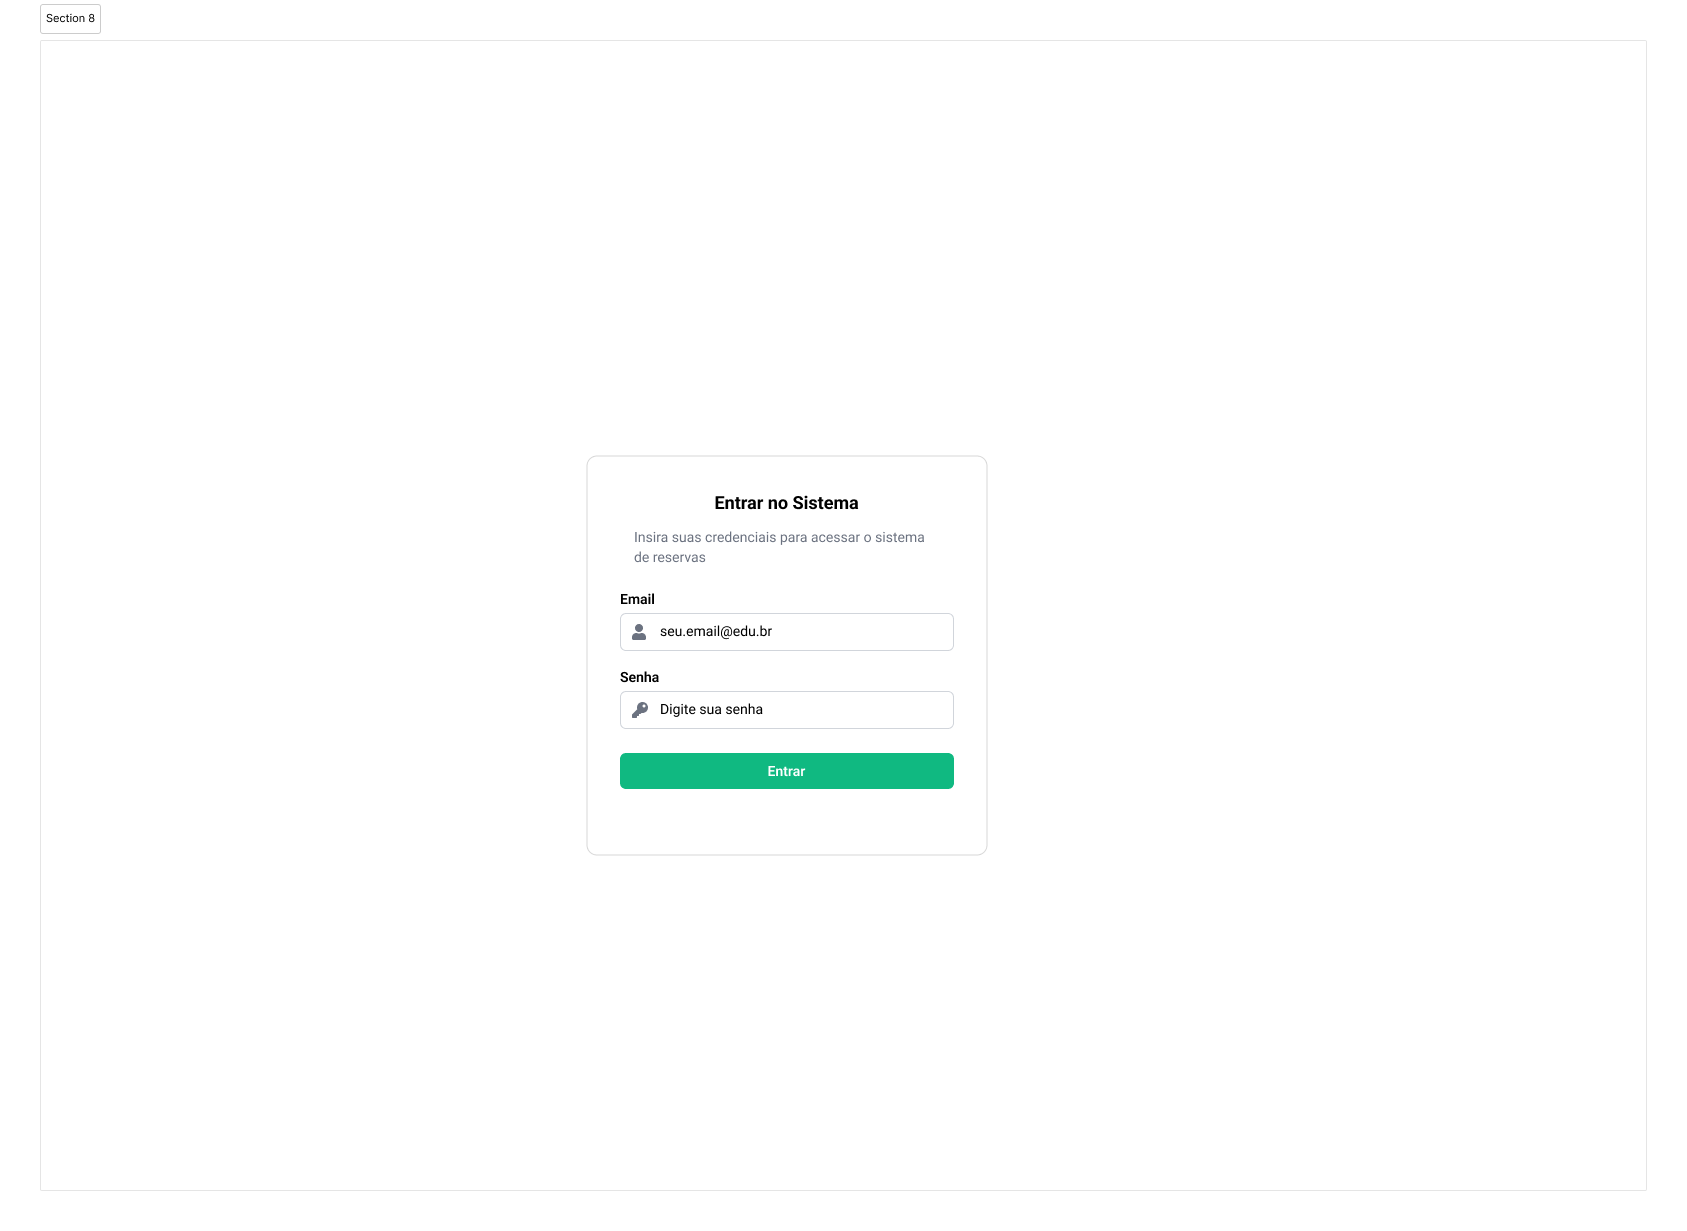
\includegraphics[width=1.5\textwidth,trim=5cm 12cm 6cm 15cm,clip]{imagens/telas/login.png}
    }
    {\footnotesize \textbf{Fonte:} O autor.}
\end{figure}

\Needspace{0.7\textheight}
\subsection{Tela de gerenciar salas}
Em Figura~\ref{fig:tela-gerenciar-salas}, o usuário pode visualizar as salas cadastradas e executar ações de gerenciamento, como adicionar, editar ou remover registros.

\begin{figure}[H]
    \caption{Tela de gerenciar salas}
    \label{fig:tela-gerenciar-salas}
    \centering
    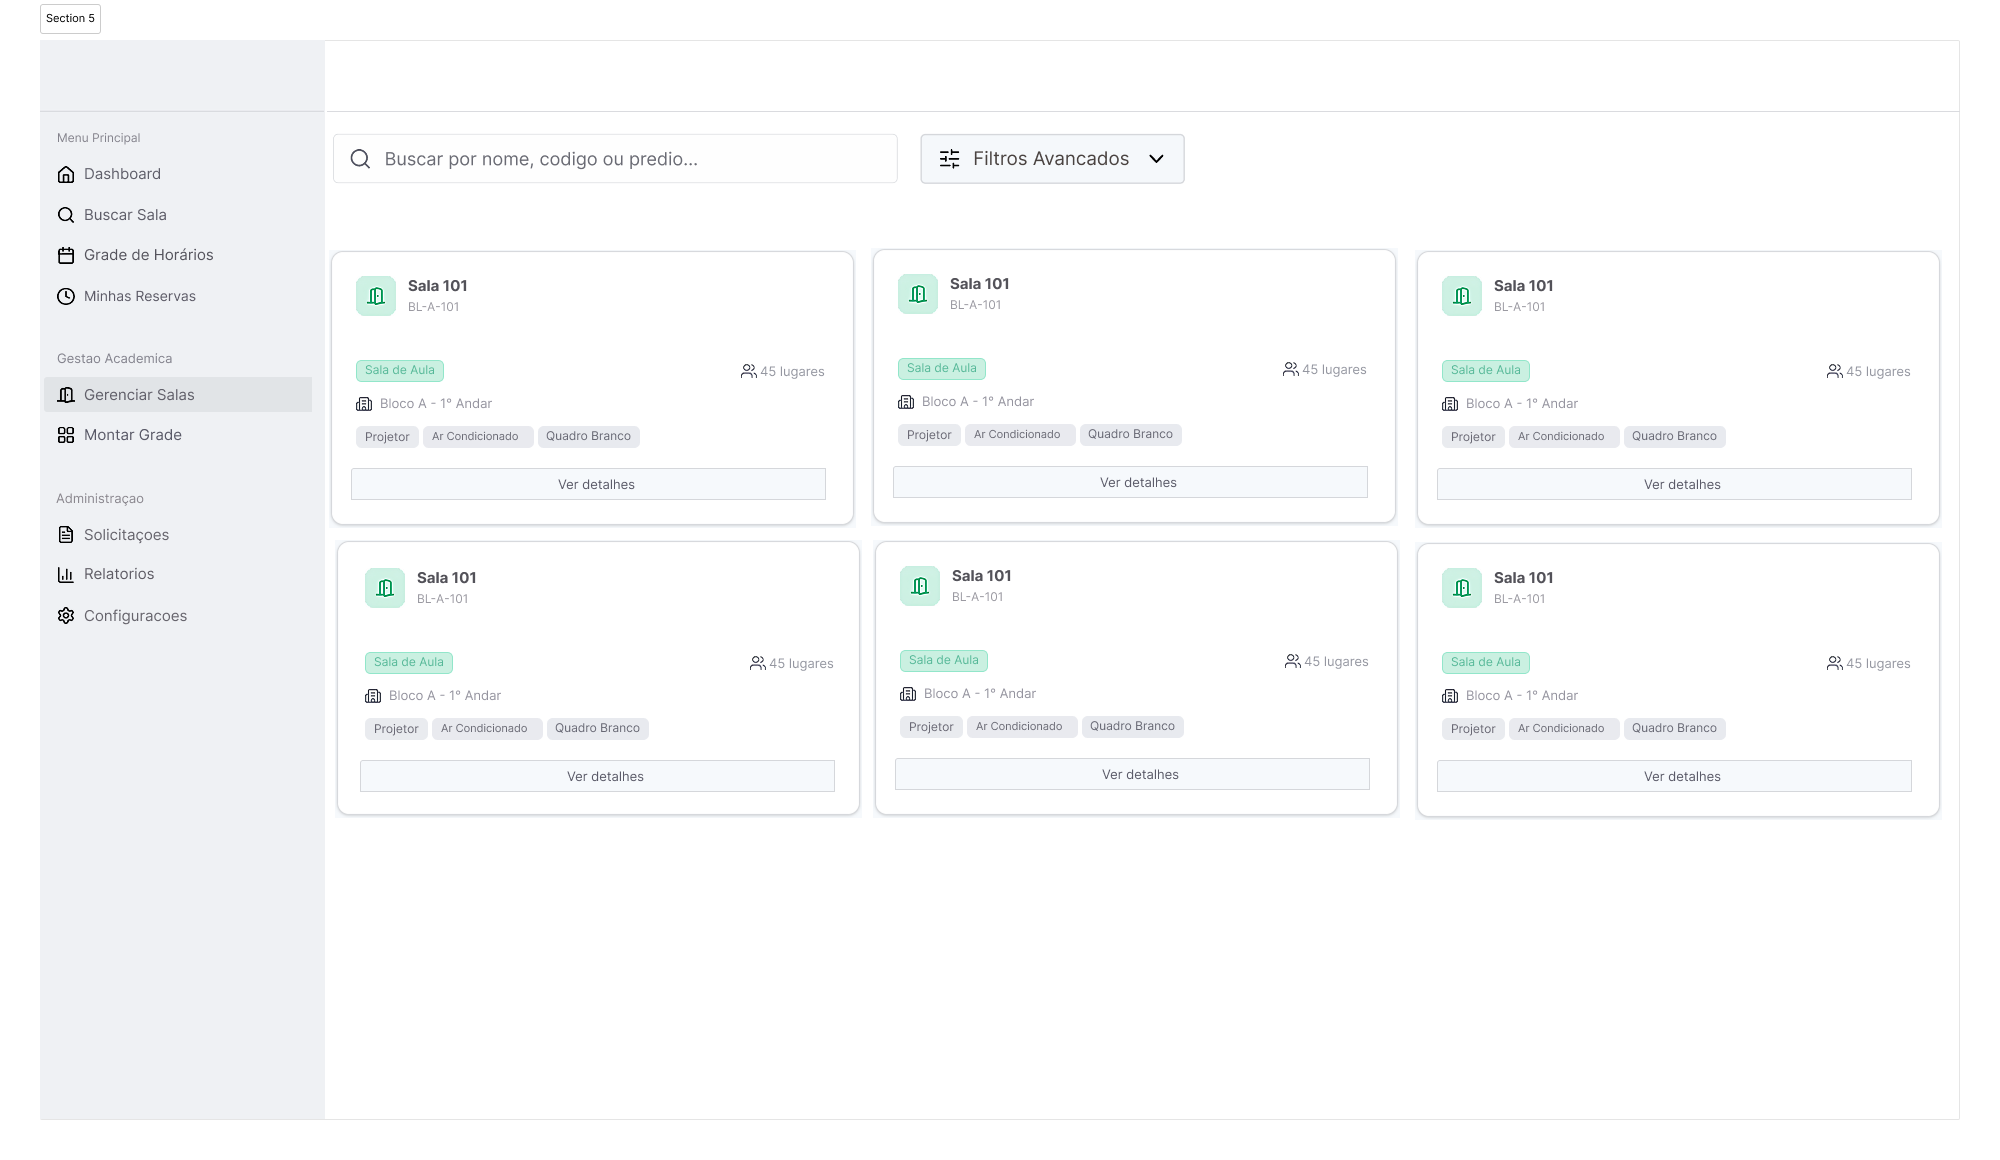
\includegraphics[width=1\textwidth]{imagens/telas/gerenciar-salas.png}
    {\footnotesize \textbf{Fonte:} O autor.}
\end{figure}

\Needspace{0.7\textheight}
\subsection{Tela de buscar sala}
Em Figura~\ref{fig:tela-buscar-sala}, esta tela permite consultar todas as salas, facilitando a localização de ambientes conforme a necessidade do usuário.

\begin{figure}[H]
    \caption{Tela de buscar sala}
    \label{fig:tela-buscar-sala}
    \centering
    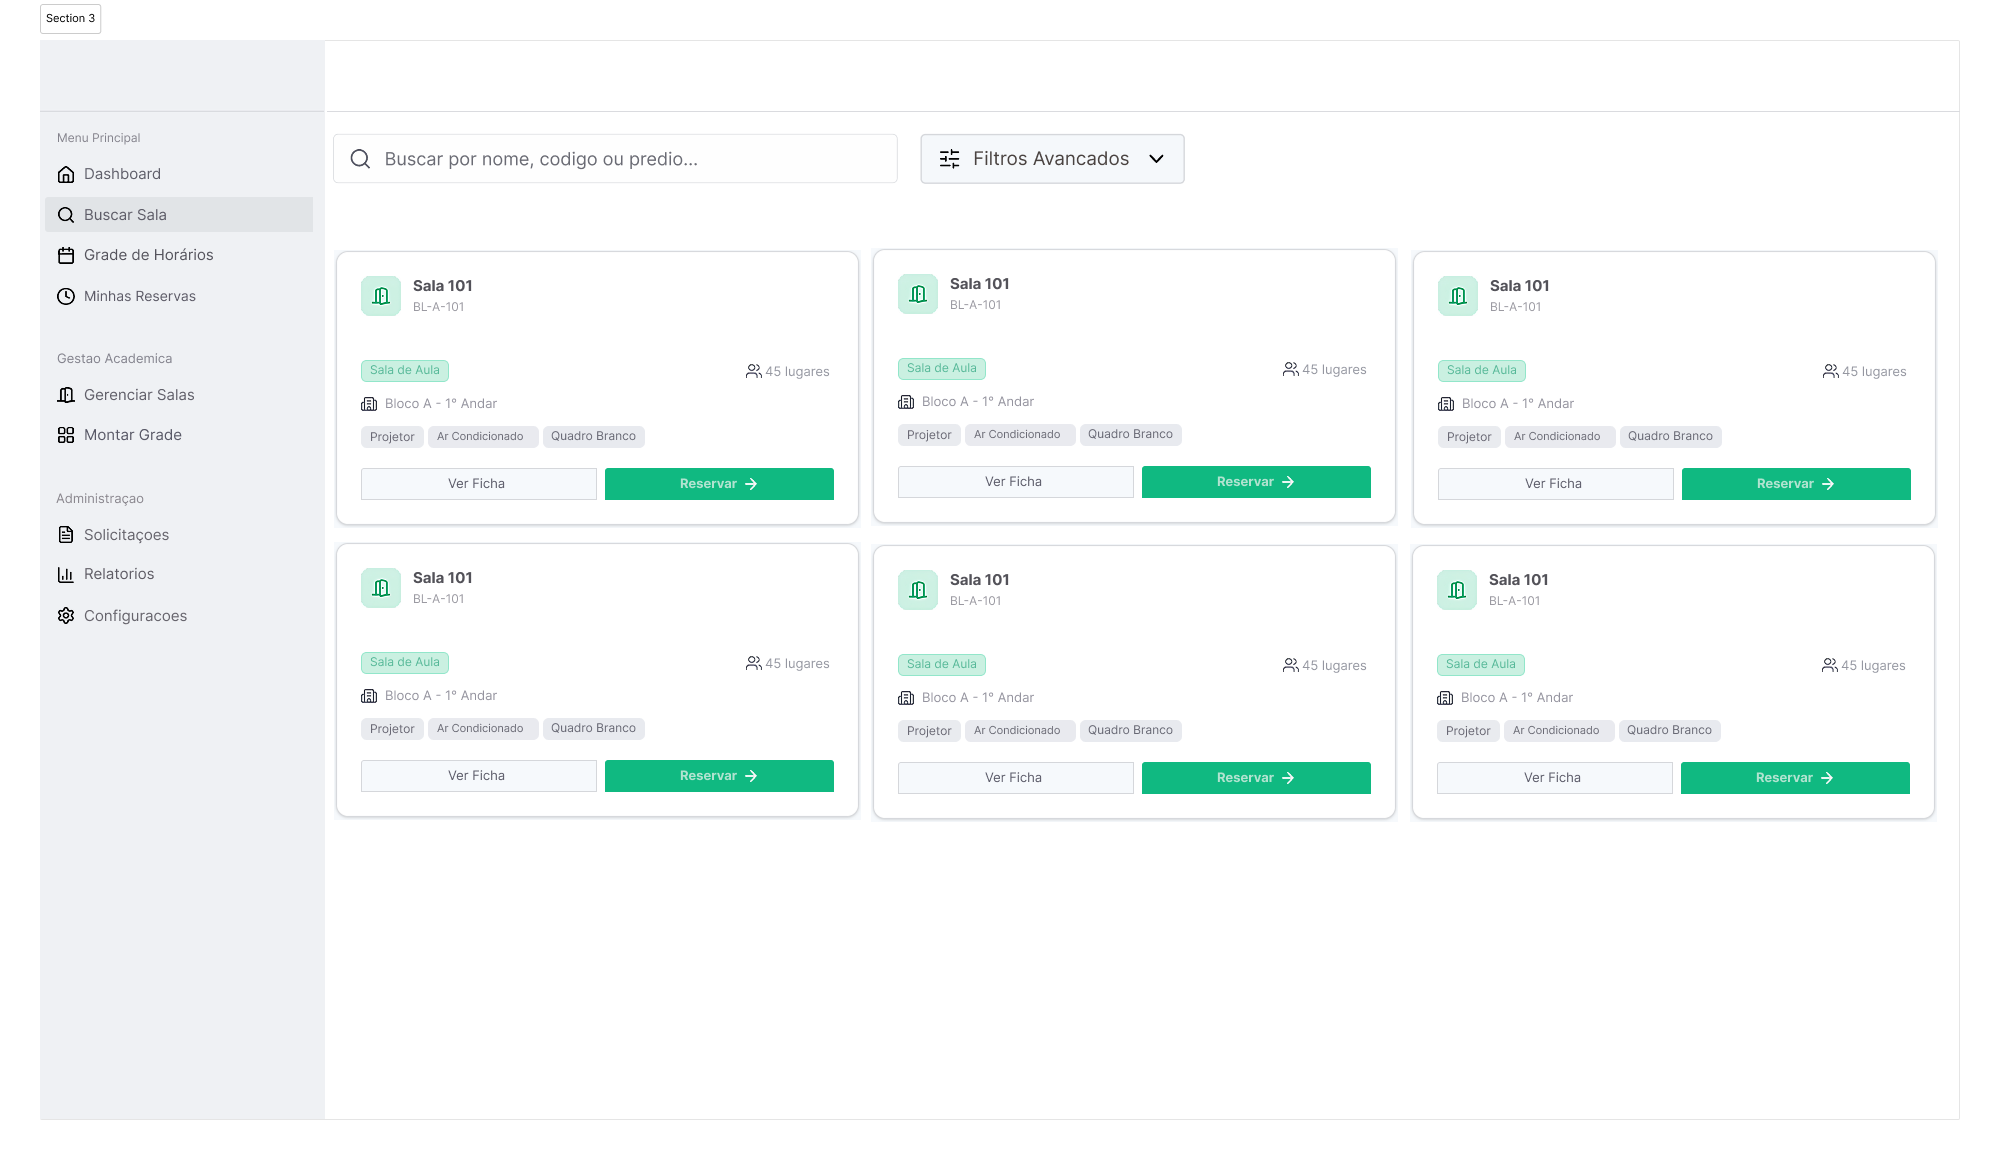
\includegraphics[width=1\textwidth]{imagens/telas/buscar-sala.png}
    {\footnotesize \textbf{Fonte:} O autor.}
\end{figure}

\Needspace{0.7\textheight}
\subsection{Tela de minhas reservas}
Em Figura~\ref{fig:tela-minhas-reservas}, o usuário acompanha as reservas realizadas, podendo consultar informações importantes sobre seus agendamentos.

\begin{figure}[H]
    \caption{Tela de minhas reservas}
    \label{fig:tela-minhas-reservas}
    \centering
    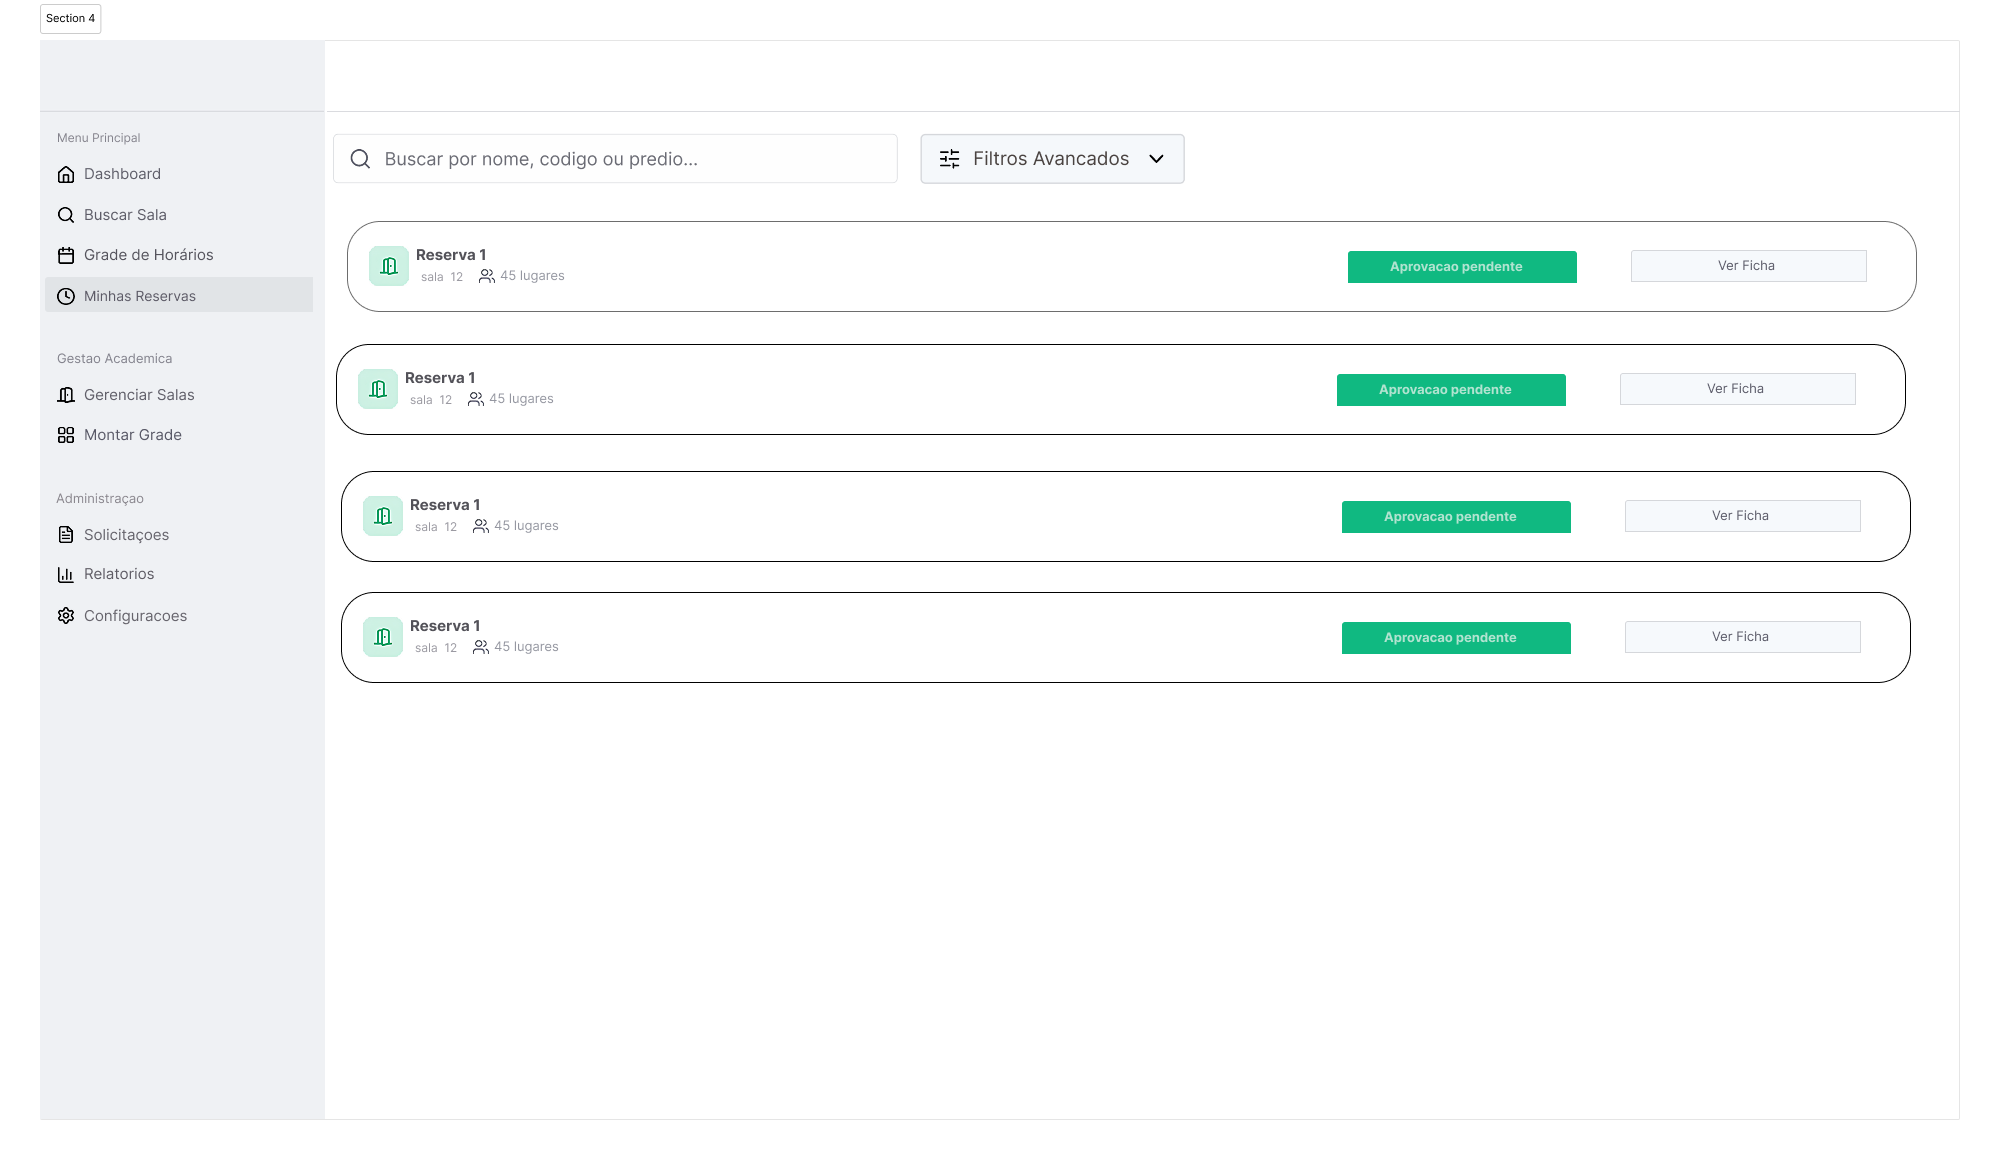
\includegraphics[width=1\textwidth]{imagens/telas/minhas-reservas.png}
    {\footnotesize \textbf{Fonte:} O autor.}
\end{figure}

\Needspace{0.7\textheight}
\subsection{Tela de solicitações}
Em Figura~\ref{fig:tela-solicitacoes}, esta tela apresenta as solicitações relacionadas ao sistema, permitindo ao usuário acompanhar pedidos e seus respectivos status.

\begin{figure}[H]
    \caption{Tela de solicitações}
    \label{fig:tela-solicitacoes}
    \centering
    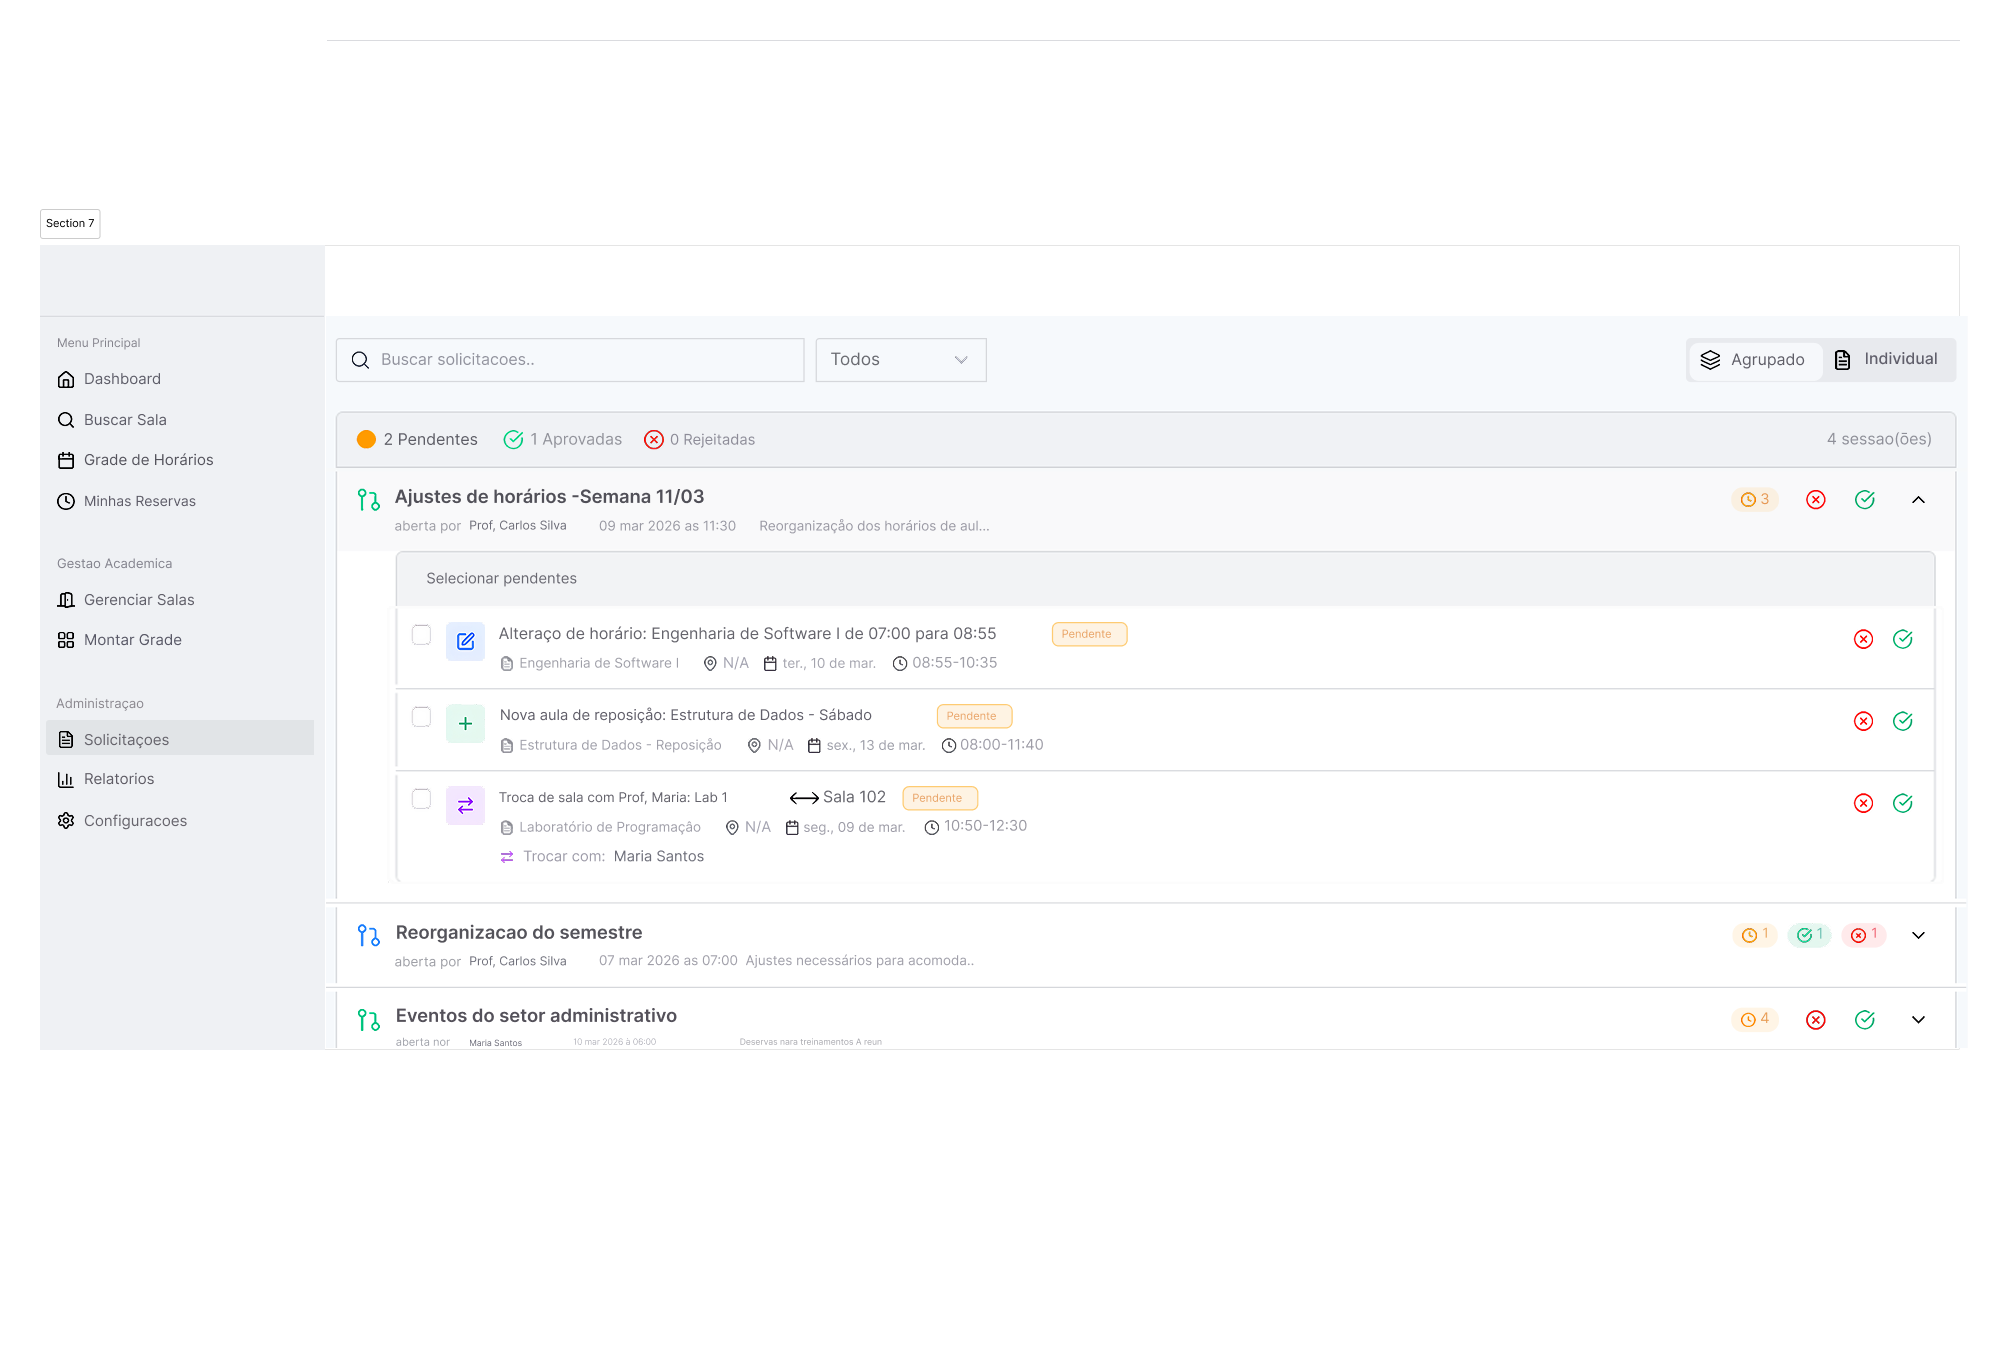
\includegraphics[width=1\textwidth]{imagens/telas/solicitacoes.png}
    {\footnotesize \textbf{Fonte:} O autor.}
\end{figure}

\Needspace{0.7\textheight}
\subsection{Tela de grade de horários}
Em Figura~\ref{fig:tela-grade-horarios}, a tela de grade de horários exibe a organização temporal das salas, ajudando na visualização da ocupação e disponibilidade.

\begin{figure}[H]
    \caption{Tela de grade de horários}
    \label{fig:tela-grade-horarios}
    \centering
    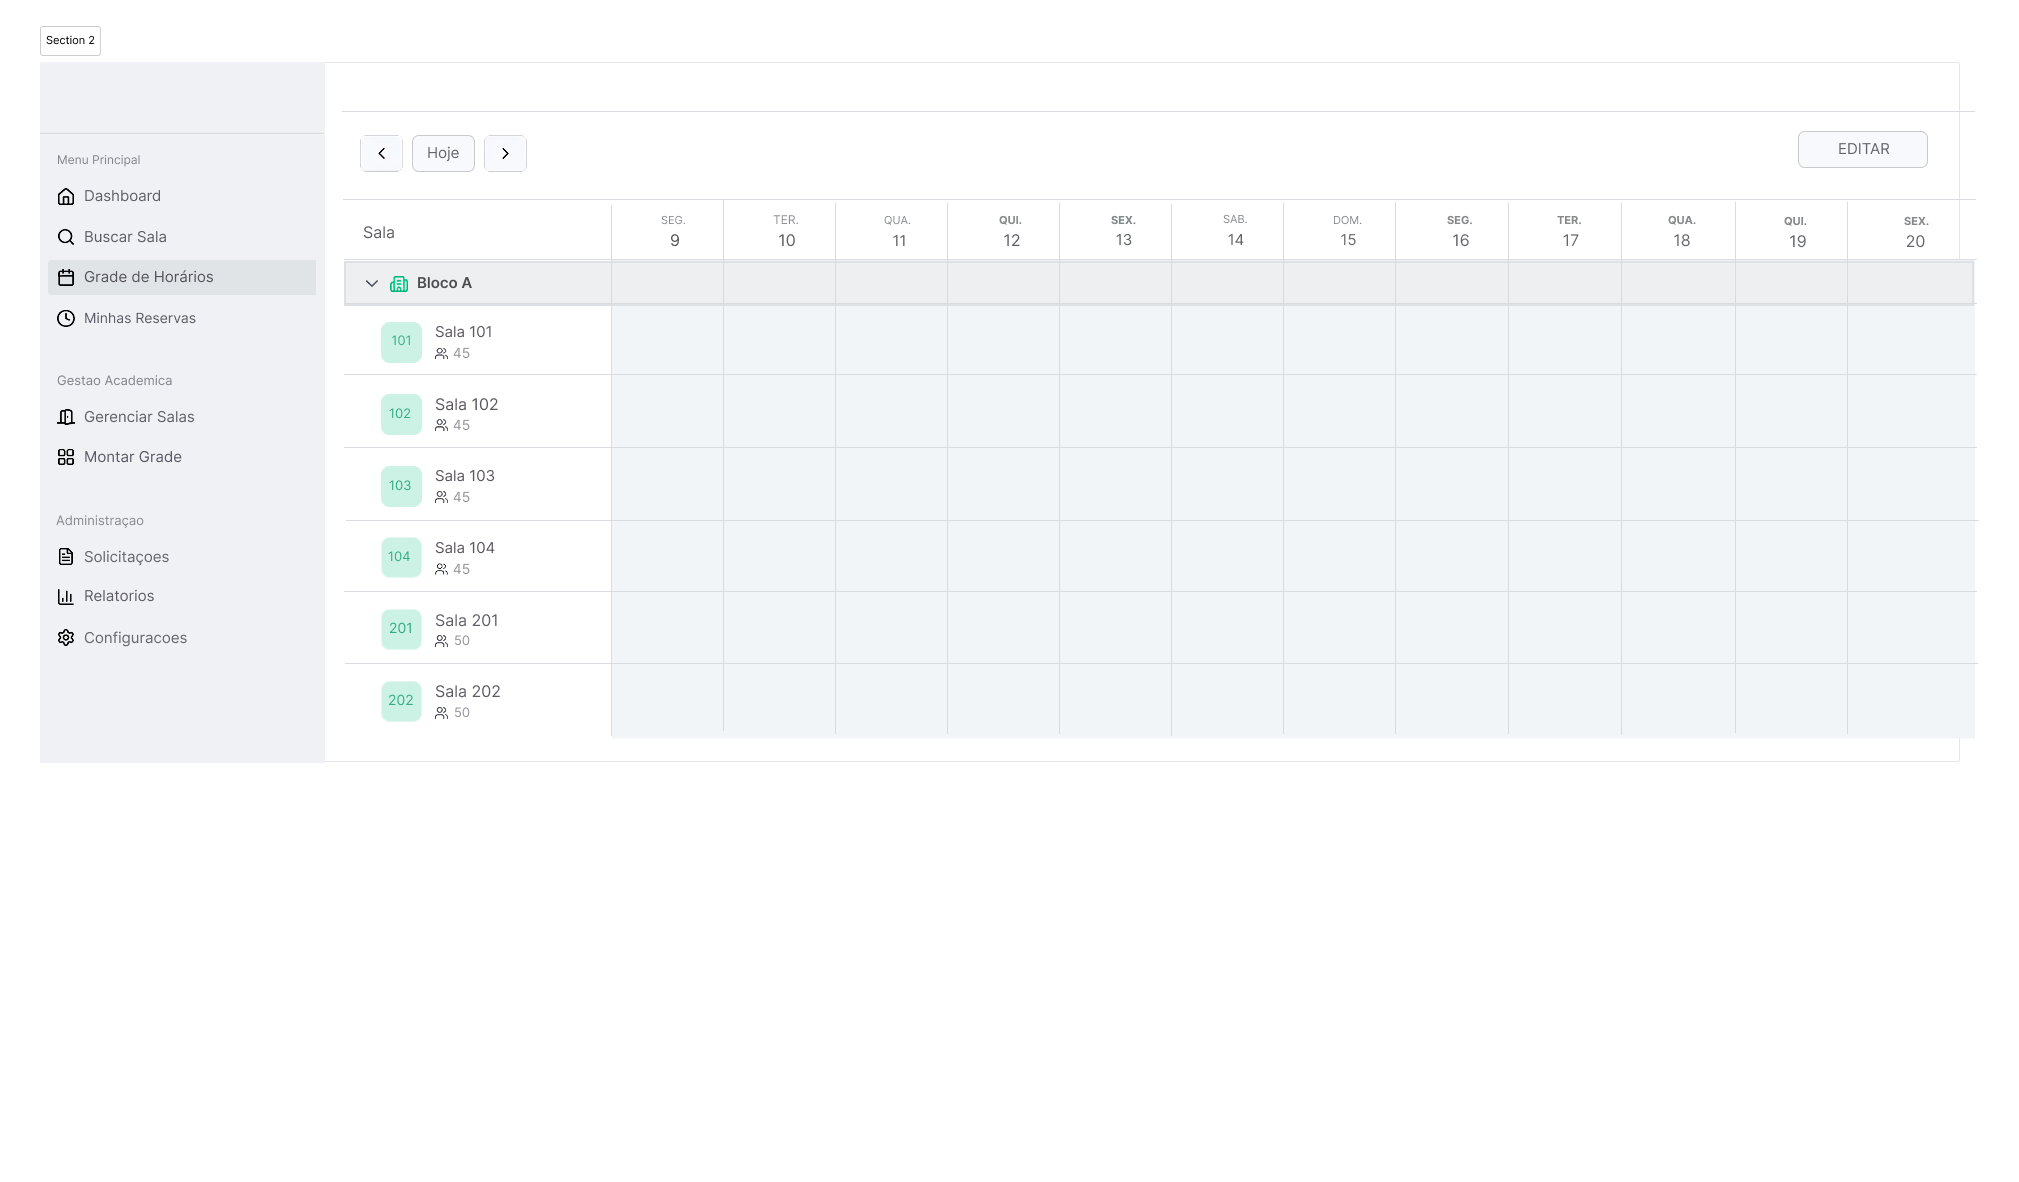
\includegraphics[width=1\textwidth]{imagens/telas/grade-horarios.png}
    {\footnotesize \textbf{Fonte:} O autor.}
\end{figure}

\chapter{Workflow (as is) na notação BPMN}\label{sec:4}

O objetivo do workflow AS-IS é representar a situação atual de um processo organizacional, o mapeando e documentando para melhor compreenção do processo como um todo. A Figura~\ref{fig:workflow-as-is} apresenta o fluxo atual de atividades do sistema.

\begin{figure}[htbp]
    \caption{Workflow AS-IS}
    \label{fig:workflow-as-is}
    \centering
    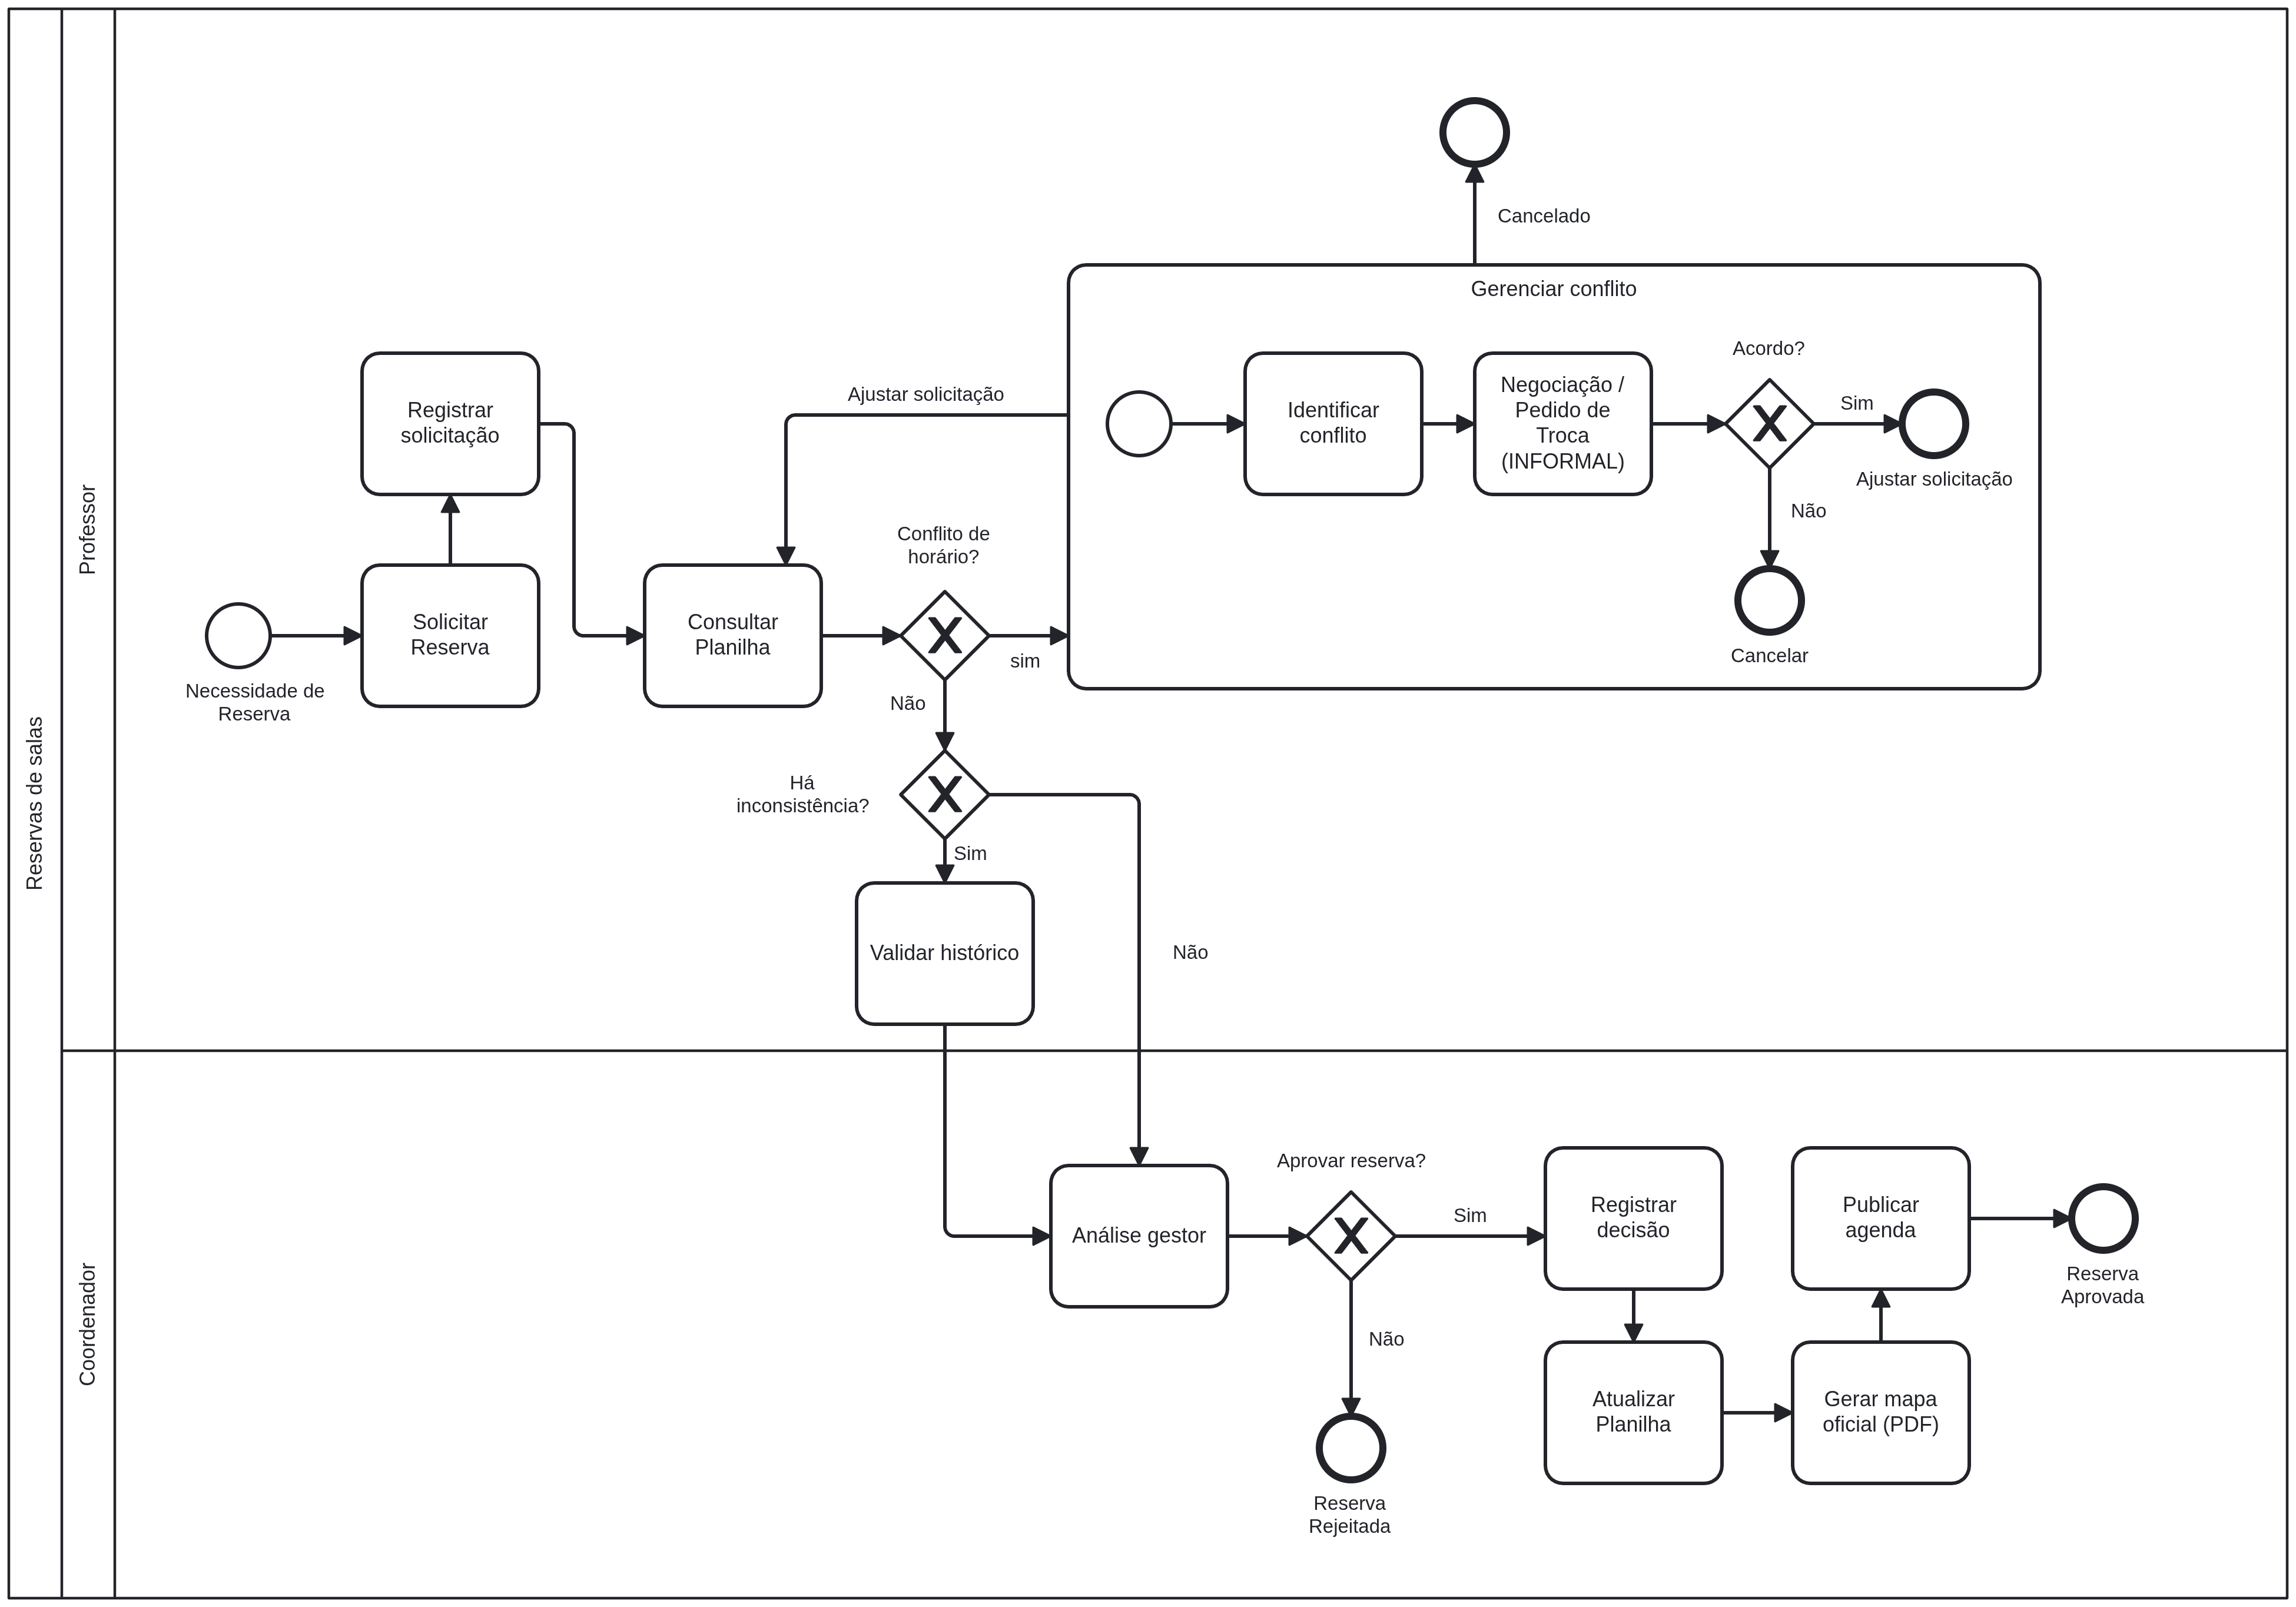
\includegraphics[width=0.8\textwidth]{imagens/workflow-as-is.png}

    {\footnotesize \textbf{Fonte:} O autor.}
\end{figure}
\chapter{Workflow (to be) na notação BPMN}\label{sec:workflow-to-be}

Enquanto o workflow AS-IS registra a situação encontrada, o workflow TO-BE representa o processo depois da introdução do sistema, servindo de referência para o que foi implementado. A Figura~\ref{fig:workflow-to-be} apresenta o fluxo proposto.

\begin{figure}[H]
    \caption{Workflow TO-BE}
    \label{fig:workflow-to-be}
    \centering
    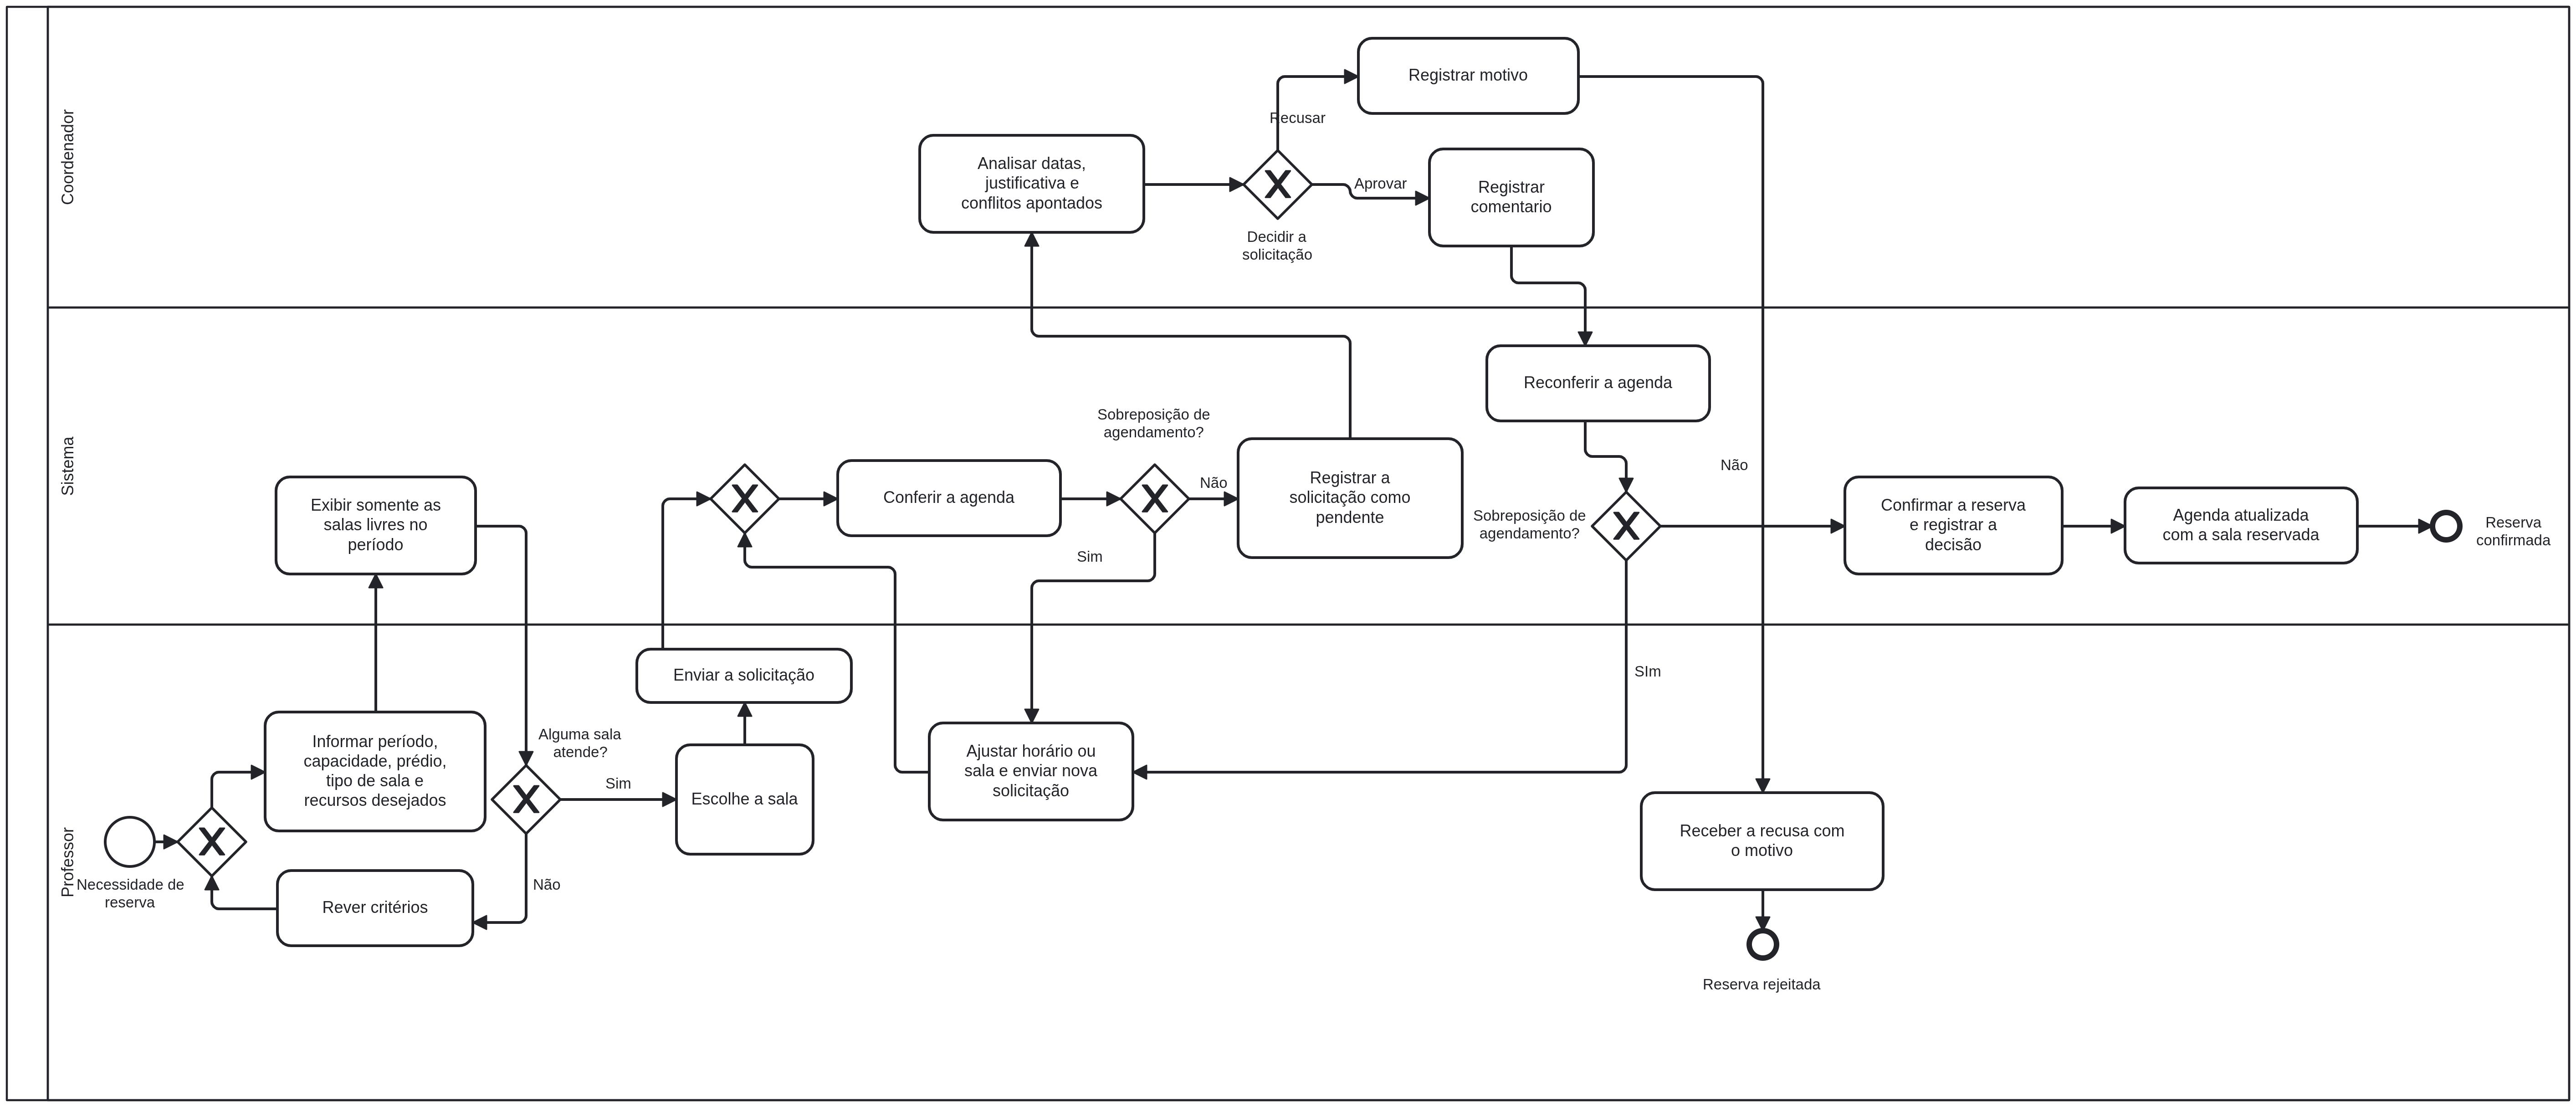
\includegraphics[width=\textwidth]{imagens/workflow-to-be.png}

    {\footnotesize \textbf{Fonte:} O autor.}
\end{figure}
\chapter{Recursos e ambiente de desenvolvimento}\label{sec:5}

Nesta seção se apresentam todas as tecnologias que serão utilizadas durante o desenvolvimento do projeto.

\section{Linguagens de Programação}

O projeto utilizará duas linguagens de programação complementares. No lado 
servidor (\textit{back-end}), será empregado o Java, linguagem 
orientada a objetos amplamente consolidada no mercado corporativo \cite{Oracle2025}. No lado 
cliente (\textit{front-end}), será utilizado o JavaScript, linguagem 
interpretada pelos navegadores web e amplamente adotada \cite{Guo2025}.

\section{Banco de Dados}

O sistema de gerenciamento de banco de dados adotado será o 
PostgreSQL \cite{PostgreSQLGlobalDevelopmentGroup2025}. A escolha se justifica pela maturidade da tecnologia e pela sua 
ampla compatibilidade com os \textit{frameworks} utilizados no projeto.

\section{\textit{Frameworks} de Desenvolvimento}

\subsection{\textit{Front-end}: React}

Para o desenvolvimento da interface do usuário, será utilizado o 
React, uma biblioteca voltada para a construção de interfaces reativas e componentizadas \cite{ReactTeam2025}. 

\subsection{\textit{Back-end}: Spring Boot}

Para o desenvolvimento da camada de negócios e exposição de APIs REST, será 
utilizado o Spring Boot, \textit{framework} baseado no ecossistema 
Spring para a plataforma Java \cite{Webb2025}.
% \chapter{Cronograma}\label{sec:6}

O cronograma é importante pois o mesmo atua como um guia que organiza as atividades, a sua principal metríca é o tempo de entrega de cada uma das atividades. A Figura~\ref{fig:conograma} apresenta o atual cronograma das atividades do projeto.

\begin{figure}[htbp]
    \caption{Conograma}
    \label{fig:conograma}
    \centering
    % O recorte segue a caixa de contorno do conteúdo do PDF, medida com
    % gs -sDEVICE=bbox: 62 59 792 528 numa página de 842x595 pt. Se a imagem
    % for trocada, remeça e ajuste, senão o recorte corta o cronograma.
    \makebox[\textwidth][c]{%
        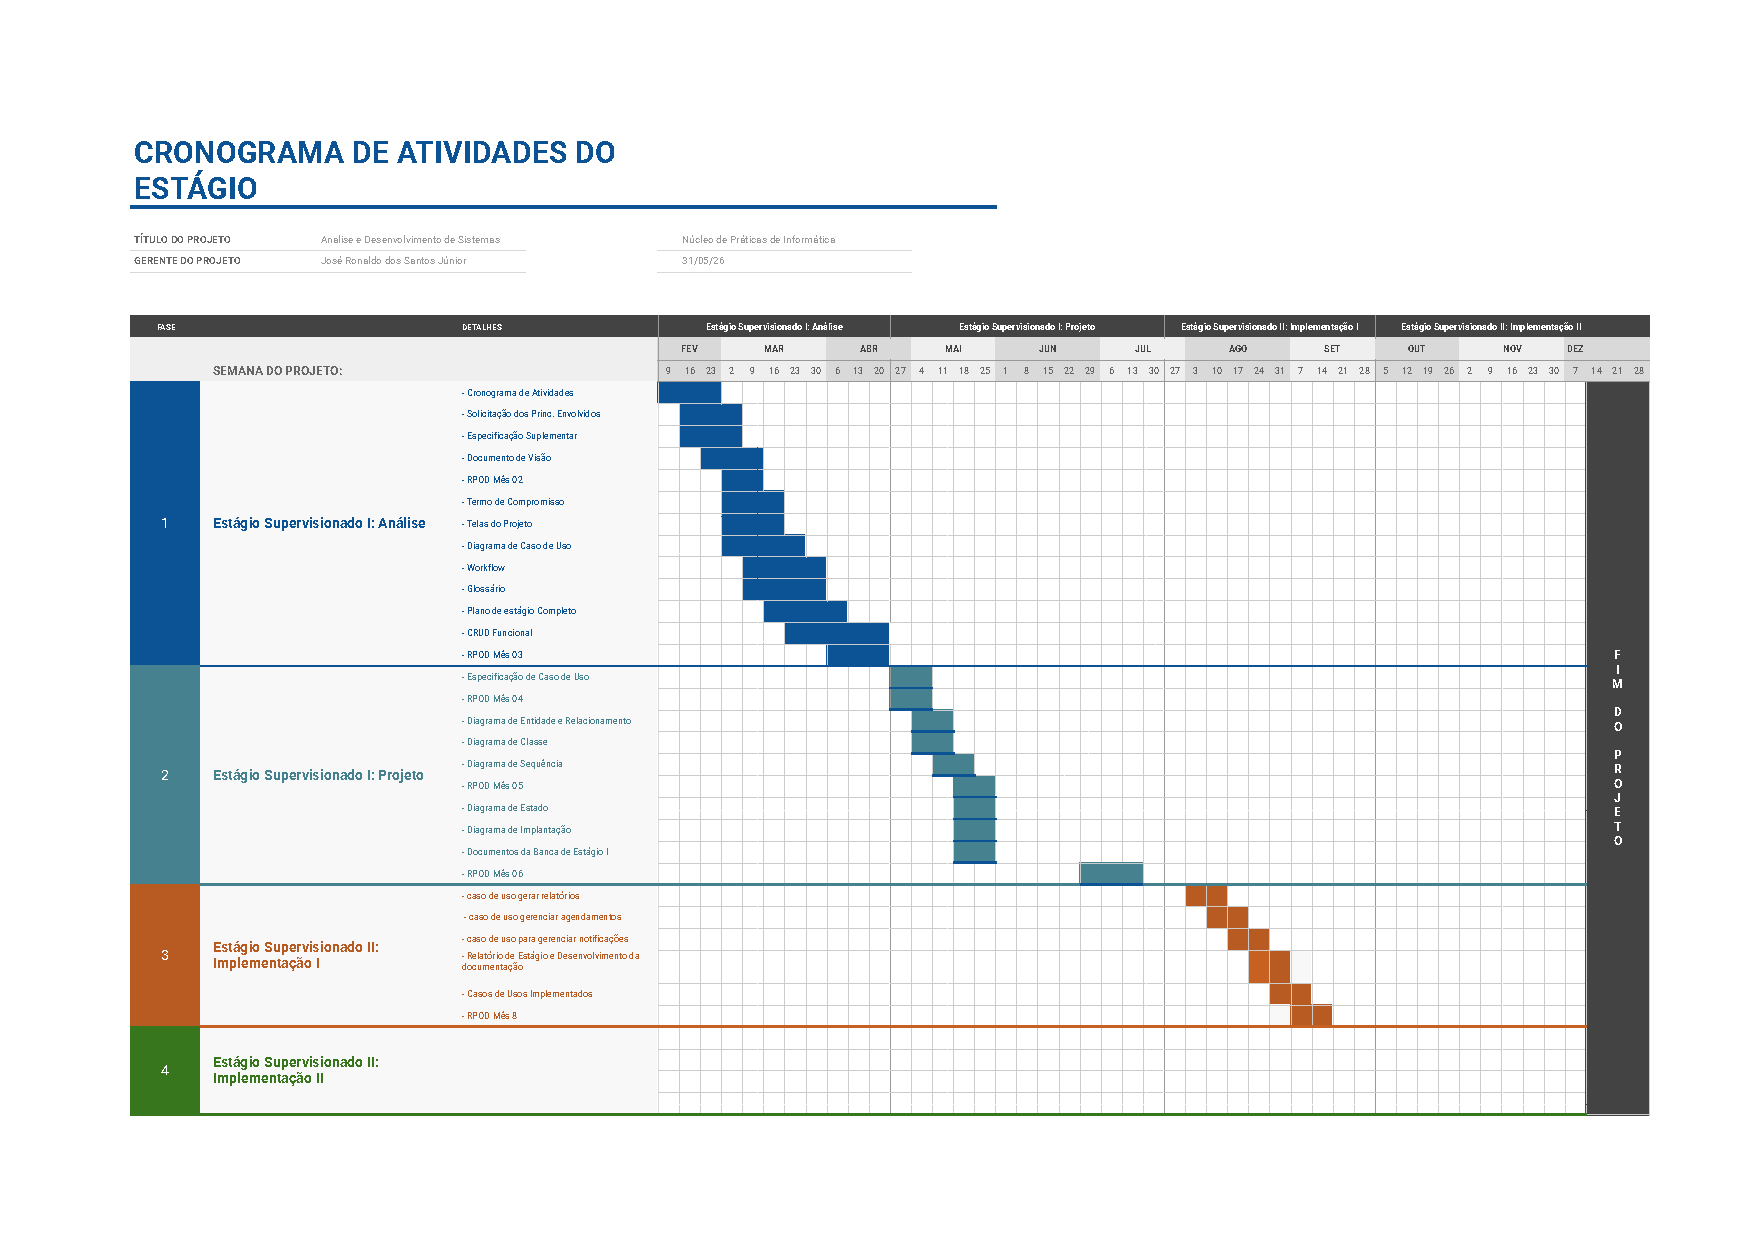
\includegraphics[width=1\textwidth,trim=60 57 48 65,clip]{imagens/CRONO.pdf}
    }
    {\footnotesize \textbf{Fonte:} O autor.}
\end{figure}

% Exemplo de utilização de bibliografia \cite{Gibson2007}.
\chapter{Conclusões e trabalhos futuros}\label{sec:conclusoes}

A realização do estágio supervisionado possibilitou o cumprimento dos objetivos propostos,
com o desenvolvimento de um sistema web de agendamento de salas para a UniFil.
A aplicação substituiu o controle feito em planilhas e estabeleceu um fluxo único
de solicitação, análise e confirmação de reservas.

Ao longo do processo foi possível aplicar na prática conceitos estudados em sala de aula,
como o levantamento de requisitos, o mapeamento de processos em BPMN e a modelagem de sistemas.
O maior desafio esteve em abstrair e gerenciar a complexidade do software,
definindo as fronteiras entre os módulos e separando a regra de negócio
do detalhe de tecnologia, o que levou a organizar a aplicação em camadas
com as dependências voltadas para o domínio.

Como possibilidade de estudos futuros, destaca-se o envio automático de notificações
sobre mudanças no status das solicitações e a geração de um relatório de grade de horários,
consolidando a ocupação das salas ao longo do semestre.
Sugere-se ainda uma funcionalidade de solicitação de troca de salas entre professores,
trazendo para dentro do sistema a negociação que hoje ocorre de maneira informal.
Mostra-se relevante também a integração com um servidor MCP (\textit{Model Context Protocol}),
permitindo que assistentes de inteligência artificial consultem a disponibilidade
e solicitem reservas.


\cleardoublepage

\postextual

%%Colocar as referências conforme as normas da ABNT, somente as utilizadas no trabalho e presentes neste manuscrito.

%Todas referências deveme star formatadas no formato .bib no arquivo bibliografia.bib para geração automática.

\bibliography{bibliografia}{}

\end{document}